Jméno:\\
Login:\\
Skupina cvičení:\\
Datum:\\

\section{Seznámení se se službou DNS}
\textbf{2.} IPv4 adresa, na kterou se překládá doménové jméno {\tt www.vutbr.cz}: \underline{\hspace{4.5cm}}
~\\
~\\
\textbf{7.} 
Autoritativní servery DNS pro doménu \texttt{vutbr.cz}:
\\
\\
\\
\\
\hspace*{0.5cm}Typ záznamů DNS, které ukazují na autoritativní servery domény:
\underline{\hspace{2cm}}
~\\
~\\
\textbf{10.} Byl proveden rekurzivní nebo iterativní dotaz DNS?
\underline{\hspace{4cm}}
\\
\\
\textbf{11.} Cílová IP adresa paketu s dotazem DNS:
\underline{\hspace{4cm}}
\\
\\
\textbf{12.} Primární e-mailový server pro doménu \texttt{fit.vutbr.cz}:
\underline{\hspace{4cm}}

\section{Seznámení se se službou Whois}
\textbf{1.} V kterém roce byla registrována doména {\tt vutbr.cz}?
\underline{\hspace{2cm}}
\\
\\
\textbf{2.} Nakonfigurovaná IPv4 adresa na rozhraní \texttt{enp2s0}: 
\underline{\hspace{3.8cm}}
\\
\\
\hspace*{0.5cm} Zjištěná veřejná IPv4 adresa: \underline{\hspace{3.8cm}}
\\
\\
\hspace*{0.5cm} Proč se veřejná adresa neshoduje s žádnou adresou nakonfigurovanou na vašem počítači?
\\
\\
\\
\textbf{3.} Do jakého rozsahu patří Vaše veřejná IP adresa?
\underline{\hspace{3.8cm}} -- \underline{\hspace{3.8cm}}
\\
\\
\hspace*{0.5cm}Komu je tento  rozsah přidělen?\hspace*{0.2cm}\underline{\hspace{3.8cm}}
\newpage
\section{Konfigurace vlastního DNS}
\textbf{14.} Výstup příkazu \texttt{nslookup 10.10.10.1}:
\\
\\
\\
\hspace*{0.7cm} Výstup příkazu \texttt{dig PCUC.xlogin00.cz}:
\\
\\
\hspace*{0.8cm}ANSWER SECTION:
\\
\\
\\
\hspace*{0.8cm}AUTHORITY SECTION:
\\
\\
\\
\hspace*{0.8cm}ADDITIONAL SECTION:
\\
\\
\\
\hspace*{0.7cm} Výstup příkazu \texttt{dig -x 10.10.10.1xx}, kde xx je číslo vašeho počítače:
\\
\\
\hspace*{0.8cm}ANSWER SECTION:
\\
\\
\\
\hspace*{0.8cm}AUTHORITY SECTION:
\\
\\
\\
\hspace*{0.8cm}ADDITIONAL SECTION:
\\
\\
\\
\textbf{17.} Doplňte sekvenční diagram modelující posloupnost dotazů DNS zachycených na rozhraních \texttt{loopback} a \texttt{enp2s0}. Do diagramu napište IP adresy serverů DNS a typy dotazů, které se při rezoluci posílají. 
\\
\\
\hspace*{0.8cm}Zadaný příkaz: \texttt{dig }\underline{\hspace{4.5cm}}
\begin{figure}[h]
	\centering
	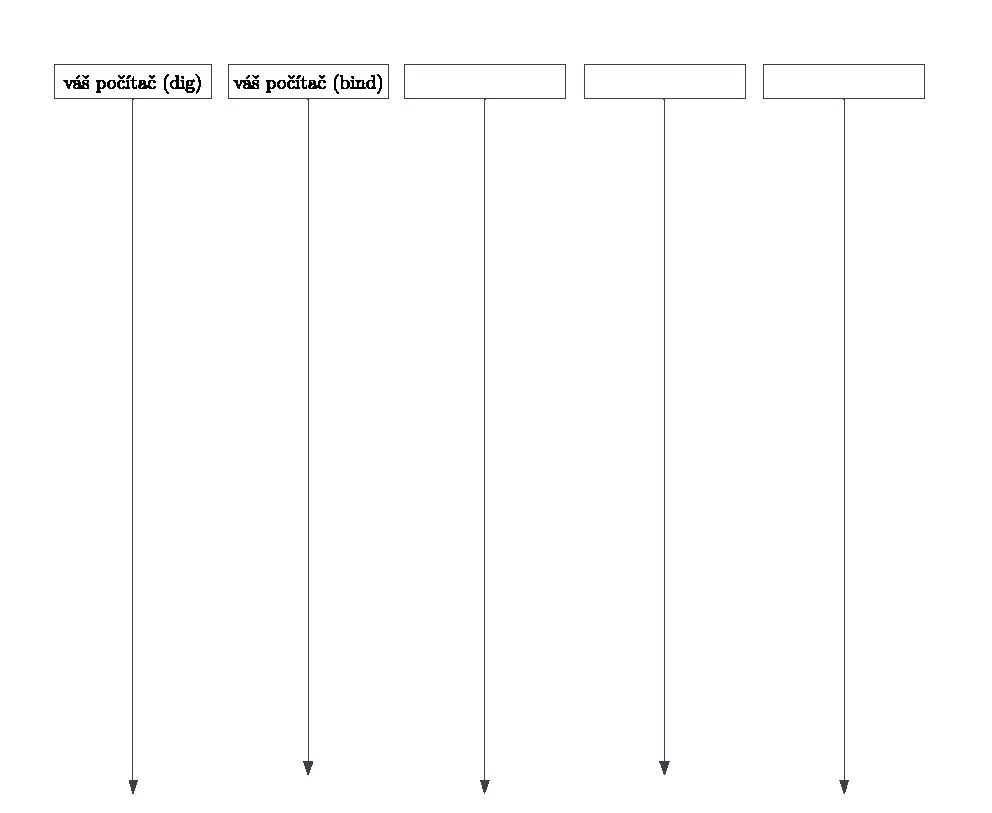
\includegraphics[bb=0 365 550 130, clip=true]{dia.eps}
\end{figure}
